\documentclass[14pt, oneside]{altsu-report}

\worktype{Отчёт по научно-исследовательской работе:}
\title{Тестер ведомых SPI устройств}
\author{Д.\,С.~Вебер}
\groupnumber{565}
\GradebookNumber{1337}
\supervisor{П.\,Н.~Уланов}
\supervisordegree{ст. пр. каф. ВТиЭ}
\ministry{Министерство науки и высшего образования}
\country{Российской Федерации}
\fulluniversityname{ФГБОУ ВО Алтайский государственный университет}
\institute{Институт цифровых технологий, электроники и физики}
\department{Кафедра вычислительной техники и электроники}
\departmentchief{В.\,В.~Пашнев}
\departmentchiefdegree{к.ф.-м.н., доцент}
\shortdepartment{ВТиЭ}
\abstractRU{	
	В ходе выполнения научно-исследовательской работы был исследован принцип работы интерфейса SPI, проведено знакомство с библиотеками для микроконтроллеров AVR и создан макет ведущего устройства. 
  
  	Цель работы --- создать макет тестера ведомых устройств, работающих по SPI интерфейсу.
  
 	 В результате выполнения научно-исследовательской работы был создан макет управляющего устройства, с помощью которого подаются различные команды ведомому устройству, работающему по SPI интерфейсу передачи данных. 
 	 }
%\abstractEN{Большой текст на английском!}
\keysRU{*}
\keysEN{computer simulation, distributed version control}

\date{\the\year}


% Подключение файлов с библиотекой.
\addbibresource{graduate-students.bib}
\usepackage{minted}
\usepackage{tocloft}
\renewcommand\cftchapfont{\mdseries}
\renewcommand\cftchappagefont{\mdseries}


\begin{document}
\maketitle
\setcounter{page}{2}
\makeabstract
\tableofcontents

\chapter*{Введение}
\addcontentsline{toc}{chapter}{Введение}
	На сегодняшний день разрабатывается достаточно много ведомых устройств, работающих по определённым интерфейсам передачи данных. Создание каждого из них занимает время как на проектирование, так и на отладку работы.
	
	Логично возникает вопрос с помощью чего устройства управляются и отлаживаются. Для такой задачи требуются ведущие устройства, которые передают данные ведомым. Поэтому разработка управляющих устройств несомненно остаётся необходимой и актуальной.
	
	В данной научно-исследовательской работе объектом обзора являются интерфейсы передачи данных, программирование микроконтроллеров. 
	
	Целью работы является создать рабочий макет тестера.
	
	Задачи научно-исследовательской работы:  
	\begin{enumerate}
		\item Выбрать инструменты разработки.
		\item Определить внешний вид макета. %TODO
		\item Разработать программу.
		\item Собрать макет.
		\item Проверить работоспособность.
	\end{enumerate}

\chapter{Обзорная глава} %TODO название

	SPI (англ. Serial Peripheral Interface, SPI bus — последовательный периферийный интерфейс, шина SPI) — последовательный синхронный стандарт передачи данных в режиме полного дуплекса, предназначенный для обеспечения простого и недорогого высокоскоростного сопряжения микроконтроллеров и периферии. Устройства, которые работают по протоколу SPI, используются в широком спектре областей, включая электронику, автомобильную промышленность, медицинское оборудование, промышленные системы и другие. Он может использоваться для передачи различных типов данных, таких как цифровые данные, команды, адреса и т.д. В зависимости от конкретной системы, которая использует протокол SPI, можно передавать следующие типы данных:
	\begin{enumerate}
		\item Цифровые данные: это наиболее распространенный тип данных, который передается по протоколу SPI. Это могут быть любые двоичные данные, например, изображения, звуковые файлы, видеофайлы, текстовые файлы и т.д.
		\item Команды: некоторые периферийные устройства могут требовать отправки команд для выполнения определенных задач. Команды могут содержать информацию о том, какое действие необходимо выполнить или какой регистр необходимо изменить.
		\item Адреса: если периферийное устройство имеет встроенную память, то адреса могут использоваться для чтения или записи данных в эту память.
		\item Управляющие сигналы: помимо данных и адресов, протокол SPI может использоваться для передачи различных управляющих сигналов, таких как сигналы часов, выборки устройств, и т.д.
	\end{enumerate}	 
	
	В целом, протокол SPI является очень гибким и может быть использован для передачи различных типов данных в зависимости от конкретной системы, которая использует этот протокол и существует множество устройств, которые могут работать в качестве SPI Master. Микроконтроллеры, такие как Arduino, Raspberry Pi или STM32, имеют встроенные контроллеры SPI, которые могут быть использованы в качестве мастера. Также на рынке существуют специальные микросхемы, такие как MAX3162 и MAX3100, которые могут быть использованы для работы в качестве SPI Master. В нашем случае устройство на базе Arduino будет передавать команды, благодаря которым можно будет выяснить, что ведомое устройство работает и выполняет поставленные требования \cite{felker2010android} \cite{wikiRUGitHub}.
	
	
	%TODO может что-то напишу ещё сюда желательно бы конечно больше текста 
	

\chapter{Создание макета устройства} %TODO стоит изменить название потом 
	Для реализации проекта была выбрана ввиду своих удобств плата на базе микроконтроллера ATmega328 --- Arduino UNO со следующими характеристиками: 
	\begin{itemize}
		\item Напряжение питания: 5 В.
		\item Цифровой ввод-вывод: 14 линий.
		\item Аналоговые входы: 6.
		\item Flash-память: 32 кб.
		\item Оперативная память: 2 кб.
		\item Встроенные интерфейсы: i2c, spi, uart, usb.
	\end{itemize}
	
		Интерфейс SPI поддерживает четыре режима работы, которые различаются настройками фазы (CPHA) и полярности (CPOL) сигнала тактирования:
	\begin{enumerate}
		\item Режим 0 (CPOL=0, CPHA=0): данные изменяются на фронте, а тактовый сигнал на спаде.
		\item Режим 1 (CPOL=0, CPHA=1): данные изменяются на спаде, а тактовый сигнал на фронте.
		\item Режим 2 (CPOL=1, CPHA=0): данные изменяются на спаде, а тактовый сигнал на фронте.
		\item Режим 3 (CPOL=1, CPHA=1): данные изменяются на фронте, а тактовый сигнал на спаде.
	\end{enumerate}
	
		В нашем устройстве интерфейс будет работать в режиме 0 и первым будет слаться младшим бит.
	
	Для разработки программы была выбрана интегрированная среда разработки Arduino IDE ввиду следующих преимуществ.
	\begin{enumerate}
		\item Простота использования: интерфейс Arduino IDE довольно прост и понятен, что делает его доступным для новичков и опытных пользователей.
		\item Бесплатное программное обеспечение: Arduino IDE является бесплатным программным обеспечением и может быть запущен на многих операционных системах.
		\item Подробная документация: документация Arduino IDE содержит множество учебных пособий, видеоуроков и примеров проектов. Это помогает пользователям легко начать работу с этой IDE.
		\item Широкое сообщество: Arduino IDE имеет очень большое количество сторонников в сообществе, которые создают новые библиотеки, расширения и советы по использованию.
	\end{enumerate}
	
	В качестве устройства ввода была выбрана клавиатура, сконструированная по способу матрицирования после чего спаяна на макетной плате размером 5х7см. Кнопки были выбраны тактовые 6x6x4.3мм в количестве двадцати штук. Шестнадцать кнопок для ввода команды и четыре для функций. 
	
	\begin{figure}[H]
	\begin{center}
	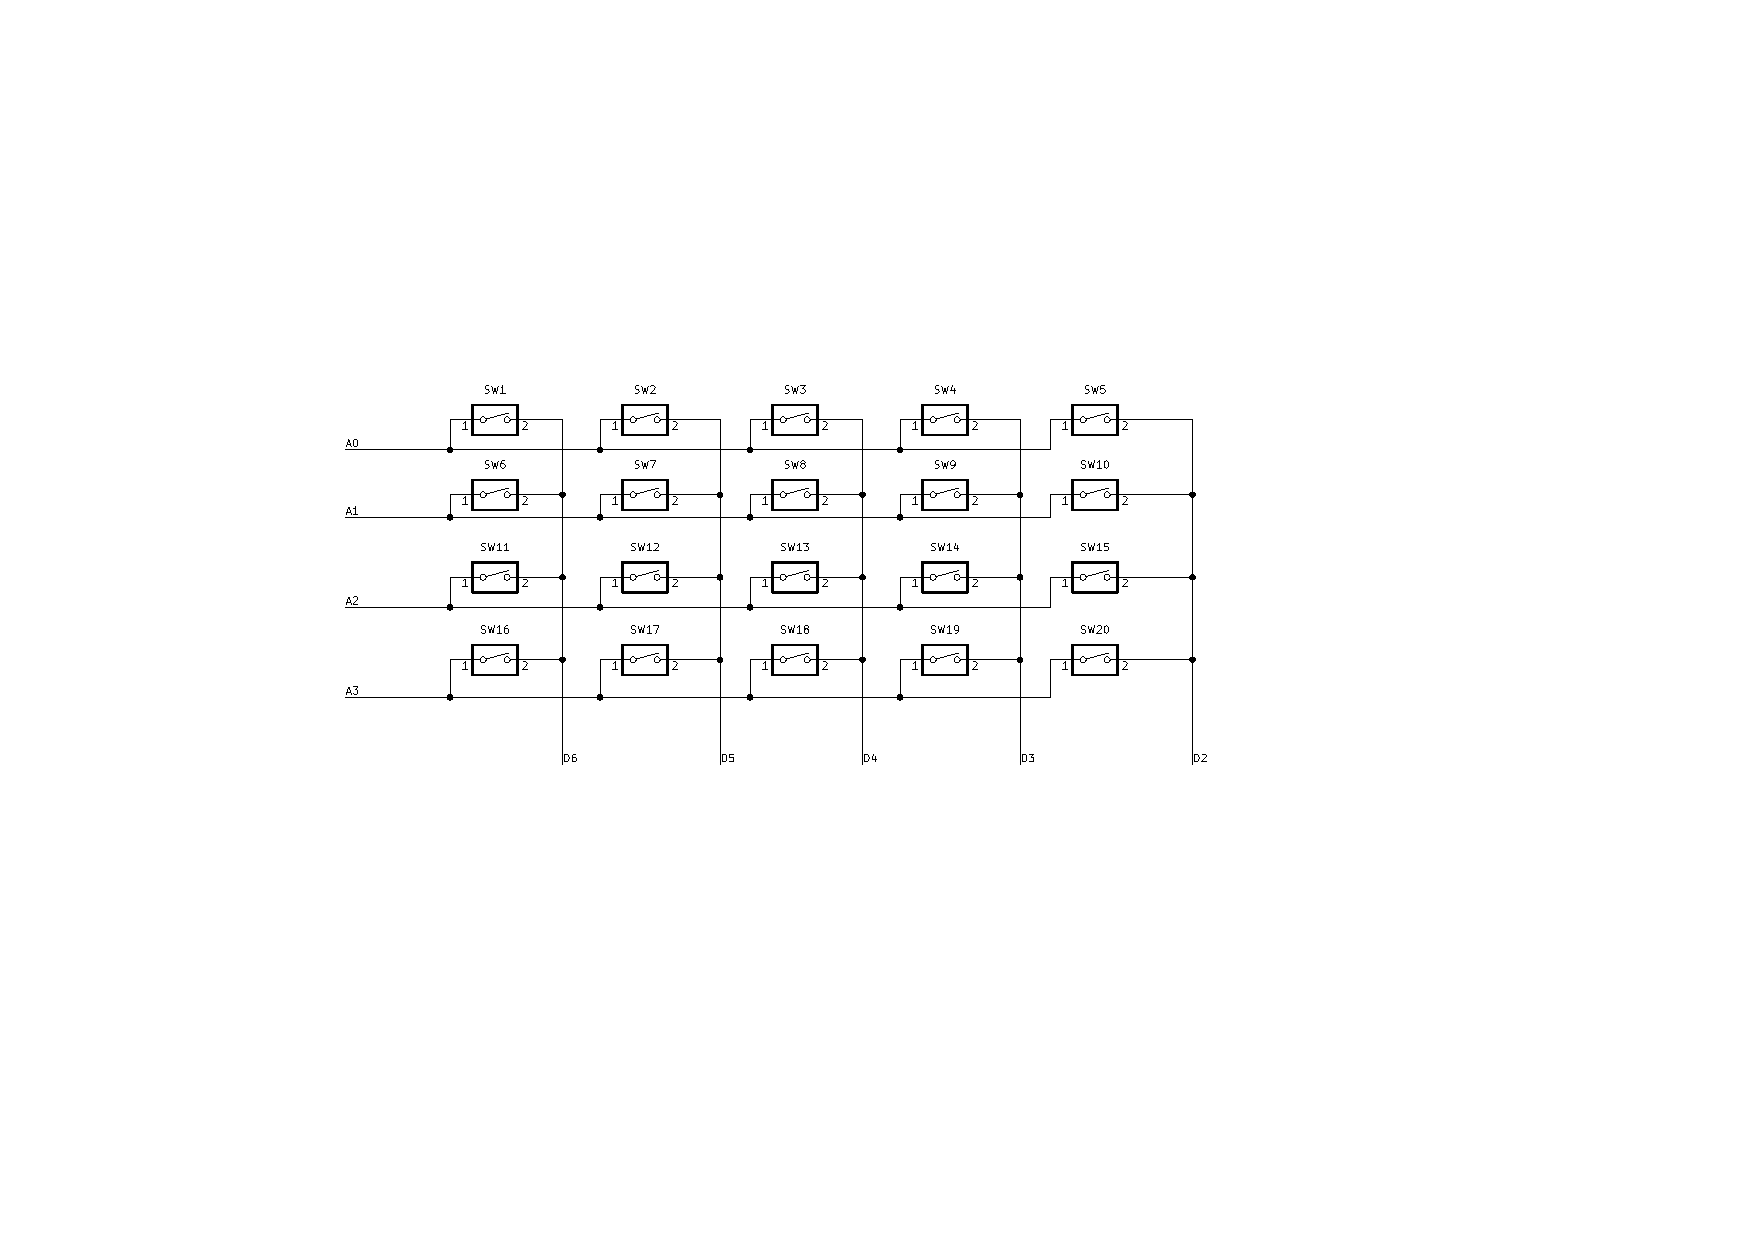
\includegraphics[scale=1]{keypad}
	\end{center}	
	\caption{Схема матричной клавиатуры}
	\end{figure}	
	
	Для обработки клавиш потребовалась библиотека. В Arduino IDE для этих целей есть <<Keypad.h>>. Эта библиотека предназначена для работы с матричными клавиатурами. Она позволяет считывать нажатия клавиш и определять, какая именно клавиша была нажата.
	После её подключения нужно определить объект класса Keypad и задать параметры его работы, такие как количество строк и столбцов, которые есть в клавиатуре. В нашем случае клавиатура 4х5. Необходимости использовать внешние резисторы или диоды нет, так как библиотека использует внутренние подтягивающие резисторы в микроконтроллере и дополнительно обеспечивает высокое входное сопротивление на всех неиспользуемых выводах столбцов.
	
	\begin{code}
	\captionof{listing}{*}
	\begin{minted}
	[
	frame=lines,
	framesep=2mm,
	baselinestretch=1.2,
	%fontsize=\footnotesize,
	linenos,
	breaklines
	]
	{text}
char keys[ROWS][COLS] = {  // раскладка клавиатуры
  { '0', '1', '2', '3', 'h' },
  { '4', '5', '6', '7', 'x' },
  { '8', '9', 'A', 'B', 's' },
  { 'C', 'D', 'E', 'F', 'd' }
};
byte rowPins[ROWS] = { A0, A1, A2, A3 };  // подключение к строкам клавиатуры
byte colPins[COLS] = { 6, 5, 4, 3, 2 };   // подключение к столбцам клавиатуры
Keypad customKeypad = Keypad(makeKeymap(keys), rowPins, colPins, ROWS, COLS); // инициализация клавиатуры
	\end{minted}
	\end{code}
	
	В листинге 2.1 мы определяем, что наша клавиатура содержит 4 строки и 5 столбцов, а также задаем, какие символы соответствуют каким клавишам. Затем мы указываем, к каким пинам на Arduino подключены строки и столбцы клавиатуры. После этого, используя метод customKeypad.getKey() считываем нажатие клавиш. 
	
	Для ввода и отправки команды потребовалось написать функцию для определения нажатой клавиши.
	
	\begin{code}
	\captionof{listing}{*}
	\begin{minted}
	[
	frame=lines,
	framesep=2mm,
	baselinestretch=1.2,
	%fontsize=\footnotesize,
	linenos,
	breaklines
	]
	{text}
void detectbuttons() {
  if (button == '0') {
    //    Serial.println("Button 0");
    if (cmd == 0)
      cmd = 0x0000;
    else
      cmd = cmd << 4;  //Pressed twice
      cmd |= 0x0000;
  }

  ...

  if (button == 'F') {
    //    Serial.println("Button F");
    if (cmd == 0)
      cmd = 0x000F;
    else
      cmd = cmd << 4;  //Pressed twice
      cmd |= 0x000F;
  }

  if (button == 's') {
    //    Serial.println("Button send");
      pack[0] = cmd;
      pack[1] = cmd >> 8;
      digitalWrite(SS, LOW);
      for (int i = 0; i < 2; i++) {
        SPI.transfer(pack[i]);
      }
      digitalWrite(SS, HIGH);
      delay(1000);
   }


  if (button == 'd') {
    //    Serial.println("Button del");
    cmd = cmd >> 4;
  }

  if (button == 'h') {  //help
    while (1) {
      myOLED.clrScr();
      myOLED.print("Help", CENTER, 0);
      myOLED.print("0 1 2 3 h", CENTER, 16);
      myOLED.print("4 5 6 7 x", CENTER, 26);
      myOLED.print("8 9 A B s", CENTER, 36);
      myOLED.print("C D E F d", CENTER, 46);
      myOLED.update();
      button = customKeypad.getKey();
      detectbuttons();
      if (button) {
        cmd = 0x00;
        break;
      }
    }
  }
	\end{minted}
	\end{code}
	
	
	В качестве устройства вывода был выбран OLED дисплей. У данного индикатора пиксели излучают свет сами, изображение получается более контрастным и насыщенным, с хорошим углом обзора. Ко всему этому у индикатора низкое энергопотребление. Имеет разрешение 128 на 64 точек, управляется по интерфейсу I2C, графический чип SSD1306 и питается от 3 --- 5 В. Для работы с ним была выбрана библиотека <<OLED\_I2C.h>> за её простоту и лёгкость. Сам же дисплей нужен для отображения команды, которую вводит пользователь.
	
	\begin{code}
	\captionof{listing}{*}
	\begin{minted}
	[
	frame=lines,
	framesep=2mm,
	baselinestretch=1.2,
	%fontsize=\footnotesize,
	linenos,
	breaklines
	]
	{text}
#include <OLED_I2C.h>
OLED myOLED(SDA, SCL);
extern uint8_t SmallFont[];
uint16_t cmd;
byte pack[2];
void setup() {
myOLED.begin();
myOLED.setFont(SmallFont);
myOLED.clrScr();
myOLED.update();
}

void loop() {
myOLED.clrScr();
myOLED.print(String(cmd, HEX), CENTER, 25);  //выводим на экран вводимую команду
myOLED.update();
}
	\end{minted}
	\end{code}
	
	Вид макета описывается следующей функциональной схемой.
	\begin{figure}[H]
	\begin{center}
	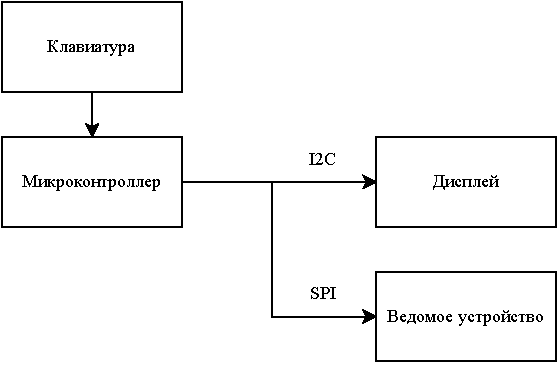
\includegraphics[scale=1]{scheme}
	\end{center}	
	\caption{Функциональная схема}
	\end{figure}	
	
		
\chapter{Описание работы устройства}
	Схему работы можно представить следующей структурной (рис.4.1) и функциональной схемами (рис. 4.2).
	\begin{figure}[H]
	\begin{center}
	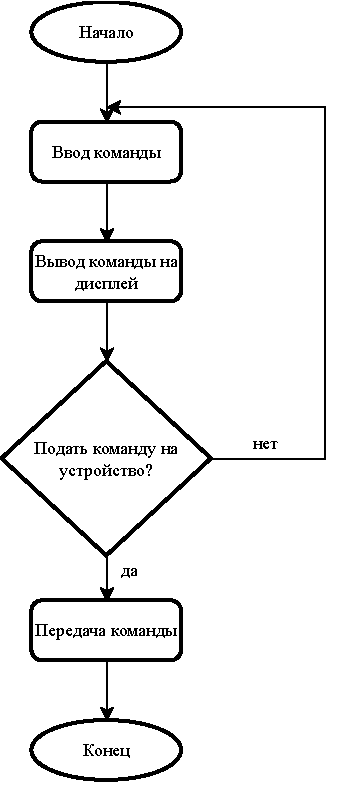
\includegraphics[scale=1]{block}
	\end{center}	
	\caption{Структурная схема}
	\end{figure}	
		

	С помощью клавиатуры пользователь вводит команду, которая передаётся на микроконтроллер, после чего она выводится на дисплей по интерфейсу I2С, затем после подтверждения передаётся на ведомое устройство по протоколу SPI.

\chapter*{Заключение}
\addcontentsline{toc}{chapter}{Заключение}
	В результате научно-исследовательской работы были выполнены следующие задачи:
	\begin{enumerate}
		\item Проведён обзор семейств микроконтроллеров и осуществлён выбор микроконтроллера для дальнейшей реализации проекта.
		\item Изучены принципы работы интерфейсов передачи данных.
		\item Рассмотрены устройства ввода-вывода для проекта.
		\item Спроектирована схема работы тестера.
	\end{enumerate}
	
	В дальнейшем предполагается применение полученных знаний для разработки собственного устройства на выбранном микроконтроллере.
\newpage
\addcontentsline{toc}{chapter}{Список использованной литературы}
\printbibliography[title={Список использованной литературы}] 

\newpage
\chapter*{\raggedleft\label{appendix1}Приложение}
\section*{Текст программы}
\begin{code}
\captionof*{listing}{*}
	\begin{minted}
	[
	frame=lines,
	framesep=2mm,
	baselinestretch=1.2,
	%fontsize=\footnotesize,
	linenos,
	breaklines
	]
	{text}
#include <SPI.h>
#include <OLED_I2C.h>
OLED myOLED(SDA, SCL);
extern uint8_t SmallFont[];
#include <Keypad.h>
const byte ROWS = 4;
const byte COLS = 5;
char button;
char keys[ROWS][COLS] = {
  { '0', '1', '2', '3', 'h' },
  { '4', '5', '6', '7', 'x' },
  { '8', '9', 'A', 'B', 's' },
  { 'C', 'D', 'E', 'F', 'd' }
};
byte rowPins[ROWS] = { A0, A1, A2, A3 };  // подключение к строкам клавиатуры
byte colPins[COLS] = { 6, 5, 4, 3, 2 };   // подключение к столбцам клавиатуры
Keypad customKeypad = Keypad(makeKeymap(keys), rowPins, colPins, ROWS, COLS);
uint16_t cmd;
byte pack[2];
void setup() {
  //Serial.begin(9600);
  pinMode(SS, OUTPUT); // настройка линии SS как выход
  SPI.begin();
  digitalWrite(SS, HIGH);
  myOLED.begin();
  myOLED.setFont(SmallFont);
  myOLED.clrScr();
  myOLED.update();
}

void loop() {
  myOLED.clrScr();
  button = customKeypad.getKey();  // определение нажатой кнопки
  if (button != NO_KEY)
    detectbuttons();
  //Serial.println(button);
  myOLED.print(String(cmd, HEX), CENTER, 25);  //выводим на экран вводимую команду
  myOLED.update();
}

void detectbuttons() {
  if (button == '0') {
    //    Serial.println("Button 0");
    if (cmd == 0)
      cmd = 0x0000;
    else
      cmd = cmd << 4;  //Pressed twice
      cmd |= 0x0000;
  }

  if (button == '1') {
    //    Serial.println("Button 1");
    if (cmd == 0)
      cmd = 0x0001;
    else
      cmd = cmd << 4;  //Pressed twice
      cmd |= 0x0001;
  }

  if (button == '2') {
    //    Serial.println("Button 2");
    if (cmd == 0)
      cmd = 0x0002;
    else
      cmd = cmd << 4;  //Pressed twice
      cmd |= 0x0002;
  }

  if (button == '3') {
    //    Serial.println("Button 3");
    if (cmd == 0)
      cmd = 0x0003;
    else
      cmd = cmd << 4;  //Pressed twice
      cmd |= 0x0003;
  }

  if (button == '4') {
    //    Serial.println("Button 4");
    if (cmd == 0)
      cmd = 0x0004;
    else
      cmd = cmd << 4;  //Pressed twice
      cmd |= 0x0004;
  }

  if (button == '5') {
    //    Serial.println("Button 5");
    if (cmd == 0)
      cmd = 0x0005;
    else
      cmd = cmd << 4;  //Pressed twice
      cmd |= 0x0005;
  }

  if (button == '6') {
    //    Serial.println("Button 6");
    if (cmd == 0)
      cmd = 0x0006;
    else
      cmd = cmd << 4;  //Pressed twice
      cmd |= 0x0006;
  }

  if (button == '7') {
    //    Serial.println("Button 7");
    if (cmd == 0)
      cmd = 0x0007;
    else
      cmd = cmd << 4;  //Pressed twice
      cmd |= 0x0007;
  }

  if (button == '8') {
    //    Serial.println("Button 8");
    if (cmd == 0)
      cmd = 0x0008;
    else
      cmd = cmd << 4;  //Pressed twice
      cmd |= 0x0008;
  }

  if (button == '9') {
    //    Serial.println("Button 9");
    if (cmd == 0)
      cmd = 0x0009;
    else
      cmd = cmd << 4;  //Pressed twice
      cmd |= 0x0009;
  }

  if (button == 'A') {
    //    Serial.println("Button A");
    if (cmd == 0)
      cmd = 0x000A;
    else
      cmd = cmd << 4;  //Pressed twice
      cmd |= 0x000A;
  }

  if (button == 'B') {
    //    Serial.println("Button B");
    if (cmd == 0)
      cmd = 0x000B;
    else
      cmd = cmd << 4;  //Pressed twice
      cmd |= 0x000B;
  }

  if (button == 'C') {
    //    Serial.println("Button C");
    if (cmd == 0)
      cmd = 0x000C;
    else
      cmd = cmd << 4;  //Pressed twice
      cmd |= 0x000C;
  }

  if (button == 'D') {
    //    Serial.println("Button D");
    if (cmd == 0)
      cmd = 0x000D;
    else
      cmd = (cmd << 4);  //Pressed twice
      cmd |= 0x000D;
  }

  if (button == 'E') {
    //    Serial.println("Button E");
    if (cmd == 0)
      cmd = 0x000E;
    else
      cmd = cmd << 4;  //Pressed twice
      cmd |= 0x000E;
  }

  if (button == 'F') {
    //    Serial.println("Button F");
    if (cmd == 0)
      cmd = 0x000F;
    else
      cmd = cmd << 4;  //Pressed twice
      cmd |= 0x000F;
  }

  if (button == 's') {
    //    Serial.println("Button send");
      pack[0] = cmd;
      pack[1] = cmd >> 8;
      digitalWrite(SS, LOW);
      for (int i = 0; i < 2; i++) {
        SPI.transfer(pack[i]);
      }
      digitalWrite(SS, HIGH);
      delay(1000);
   }

  if (button == 'd') {
    //    Serial.println("Button del");
    cmd = cmd >> 4;
  }

  if (button == 'h') {  //help
    while (1) {
      myOLED.clrScr();
      myOLED.print("Help", CENTER, 0);
      myOLED.print("0 1 2 3 h", CENTER, 16);
      myOLED.print("4 5 6 7 x", CENTER, 26);
      myOLED.print("8 9 A B s", CENTER, 36);
      myOLED.print("C D E F d", CENTER, 46);
      myOLED.update();
      button = customKeypad.getKey();
      detectbuttons();
      if (button) {
        cmd = 0x00;
        break;
      }
    }
  }
}
	\end{minted}
	\end{code}
\end{document}

